%----
\subsection{Activity}
\textbf{Activity} --- одно окно приложения.

\begin{itemize}
	\item может занимать весь экран или его часть;
	\item может быть запущена из других компонент приложения или из другого приложения;
	\item может возвращать результат.
\end{itemize}

\begin{figure}[H]
    \centering
    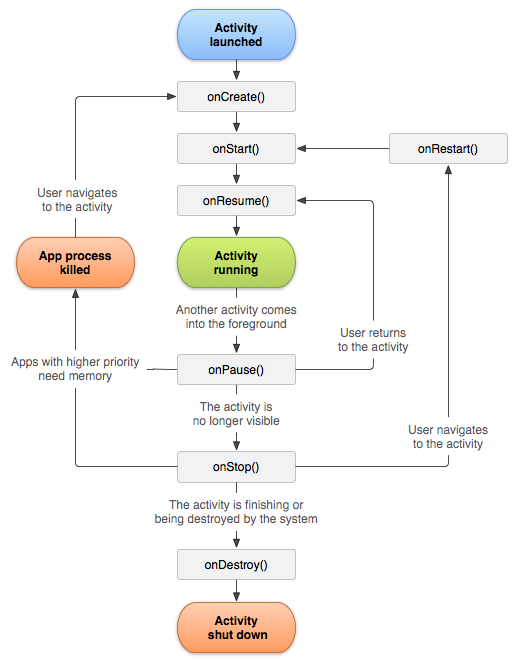
\includegraphics[width=0.5\textwidth]{activity_lifecycle}
    \caption{Жизненный цикл Activity}
    \label{fig:activity_lifecycle}
\end{figure}

На разных этапах существования Activity андроид вызывает различные методы, основные представлены на рисунке \ref{fig:activity_lifecycle}.

\begin{itemize}
	\item \textit{onCreate()} --- вызывается первым. В нем как правило создаются UI контролы.
	\item \textit{onStart()} --- вызывается в момент появления Activity на экране.
	\item \textit{onResume()} --- вызывается когда пользователь начинает взаимодействовать с Activity.
	\item \textit{onPause()} --- вызывается когда пользователь заканчивает работать с Activity. Если приложение осталось на экране и пользователь в дальнейшем возвращается обратно, идет вызов \textit{onResume()}.
	\item \textit{onStop()} --- вызывается когда Activity полностью уходит с экрана и перестает быть видимым.
	\item \textit{onRestart()} --- вызывается при возврате в Activity и далее \textit{onStart()}.
	\item \textit{onDestroy()} --- вызывается при сммене конфигурации или если пользователь закрыл Activity. Activity уничтожается.
\end{itemize}

Приложение может быть уничтожено после методов \textit{onPause()}, \textit{onStop()}. В этом случае следующие методы вызваны не будут, например \textit{onDestroy()}. За освобождение ресурсов при этом отвечает уже ОС.

\begin{figure}[H]
    \centering
    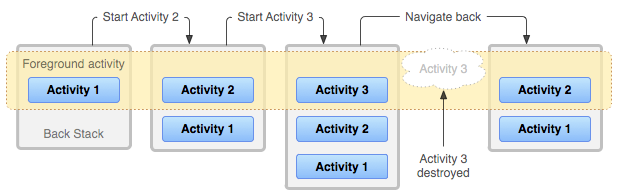
\includegraphics[width=0.8\textwidth]{diagram_backstack}
    \caption{Activity back stack}
    \label{fig:diagram_backstack}
\end{figure}

Как правило в приложении существует не одно Activity, а несколько. Когда пользователь вызывает из одной Activity другую, оно кладется сверху, а первая Activity уходит вниз (см. рисунок ). Таким образом образуется некий стек Activity. Когда пользователь нажимает кнопку \textit{back}, с этого стека верхняя Activity сносится, уничтожается и наверх поднимается та, что была под ней.

На рисунке \ref{fig:diagram_backstack} изображено поведение \textit{back stack} по умолчанию, которое можно изменять.

Для изменения поведения \textit{back stack} в Activity существует параметр \textit{Launch Modes}.
\begin{itemize}
	\item \textit{standart (default mode)} --- при каждом запуске Activity создается новый экземпляр Activiy и помещается на вершину \textit{back stack};
	\item \textit{singleTop} --- если в момент запуска экземпляр Activity уже находится на вершине стека, то новый экземпляр не создается, вместо этого вызывается метод \textit{onNewIntent()} у существующего экземпляра;
	\item \textit{singleTask} --- Activity запускается в отдельном \textit{Task}. Если экземпляр Activity уже существует, то у него вызывается метод \textit{onNewIntent()}, а все Activity лежащие в \textit{back stack} поверх этого экземпляра - уничтожаются.
	\item \textit{singleInstance} то же, что и \textit{singleTask}, но Activity является в своем таске единственной.
\end{itemize}


%----
\subsubsection{Пересоздание Activity}
	Android пересоздает Activity:
	\begin{itemize}
		\item при изменении конфигурации устройства, например когда изменяется ориентация экрана, пользователь меняет язык системы в настройках Android и т.п.;
		\item при возврате пользователя к процессу, который был убит Android для освобождения ресурсов.
	\end{itemize}
	
	
%----	
\subsubsection{Сохранение состояния при пересоздании Activity}

	\begin{figure}[H]
	    \centering
	    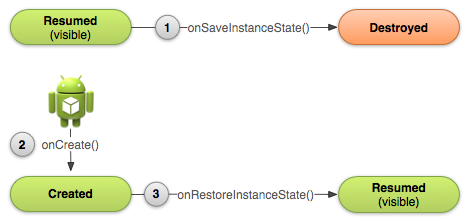
\includegraphics[width=0.8\textwidth]{basic_lifecycle_savestate}
	    \caption{Сохранение состояния при пересоздании Activity}
	    \label{fig:basic_lifecycle_savestate}
	\end{figure}
	
	\lstset{
	    language=java,
	    caption=Пример сохранения состояния при пересоздании Activity,
	    label=code:basicLifecycleSavestate_java,
	    keywordstyle=\color{blue}\bf,
	    commentstyle=\color{OliveGreen},
	    stringstyle=\color{red},
	    basicstyle=\scriptsize   
	}
	
	\lstinputlisting{files/basicLifecycleSavestate.java}
	
Если на Activity есть, например, EditText элемент в который пользователь может вбить свои строки, то нет необходимости специально сохранять этот текст, а достаточно вызвать суперметод в \textit{onSaveInstanceState}, либо не перекрывать его вообще. Отключить сохранение можно в свойствах элемента EditText.

Но таким образом сохранаются не все параметры элементов. Например, свойство \textit{visibility} не сохраняется и его можно сохранить отдельно (см. пример кода \ref{code:basicLifecycleSavestate_java}).

Не все объекты можно и нужно сохранять в \textit{Bundle}. Например, большие объемы данных будут сохраняться очень долго. 


%----	
\subsubsection{Сохранение объекта при пересоздании Activity}

\begin{itemize}
	\item методы \textit{onRetainNonConfigurationInstance / \newline getLastNonConfigurationInstance} --- \textbf{не рекомендуется};
	\item \textit{Static Field/Singleton/Application object}. \newline \textit{Singleton} --- существует один для всех экземпляров Activity, что может привести к проблемам, также не уничтожается вместе с Activity;
	\item \textit{Service} --- принципиально не отличается от \textit{Singleton}, но имеет дополнительные проблемы из-за асинхронности подключения к Activity;
	\item \textit{Retain Instance Fragment}.
\end{itemize}